%%
%% This is file `sample-sigconf.tex',
%% generated with the docstrip utility.
%%
%% The source files were:
%%
%% samples.dtx  (with options: `all, proceedings,bibtex,sigconf')
%% 
%% IMPORTANT NOTICE:
%% 
%% For the copyright, see the source file.
%% 
%% Any modified versions of this file must be renamed
%% with new filenames distinct from sample-sigconf.tex.
%% 
%% For distribution of the source, see the terms
%% for copying and modification in the file samples.dtx.
%% 
%% This generated file may be distributed as long as the
%% source files, as listed above, are part of the
%% same distribution. (The sources need not necessarily be
%% in the same archive or directory.)
%%
%%
%% Commands for TeXCount
%TC:macro \cite [option:text,text]
%TC:macro \citep [option:text,text]
%TC:macro \citet [option:text,text]
%TC:envir table 0 1
%TC:envir table* 0 1
%TC:envir tabular [ignore] word
%TC:envir displaymath 0 word
%TC:envir math 0 word
%TC:envir comment 0 0
%%
%% The first command in your LaTeX source must be the \documentclass
%% command.
%%
%% For submission and review of your manuscript please change the
%% command to \documentclass[manuscript, screen, review]{acmart}.
%%
%% When submitting camera ready or to TAPS, please change the command
%% to \documentclass[sigconf]{acmart} or whichever template is required
%% for your publication.
%%
%%
\documentclass[sigconf,nonacm]{acmart}
  % Hides ACM Reference Format box
%%
 \settopmatter{printacmref=false}  
 \setcopyright{none}              % disables copyright notice

\renewcommand\footnotetextcopyrightpermission[1]{} % suppresses first-page footer
\fancyhead{}  % Remove header content
\fancyfoot{}                     % clears footer content% Removes citation info below abstract
% Override conference info manually with blank text
 \usepackage{float}
\usepackage{balance} 
\usepackage{booktabs}
\usepackage{makecell}
\usepackage{float}
\usepackage{balance} 
\usepackage{adjustbox} 
\usepackage{tabularx}
\usepackage{tikz}
\usepackage[table]{xcolor} % Add to your preamble
\usepackage[compact]{titlesec}
\usepackage{subcaption} % For subfigure environment
%% \BibTeX command to typeset BibTeX logo in the docs
\AtBeginDocument{%
  \providecommand\BibTeX{{%
    Bib\TeX}}}
\usepackage{enumitem}

%% Rights management information.  This information is sent to you
%% when you complete the rights form.  These commands have SAMPLE
%% values in them; it is your responsibility as an author to replace
%% the commands and values with those provided to you when you
%% complete the rights form.
 
%% These commands are for a PROCEEDINGS abstract or paper.
 
%%
%%  Uncomment \acmBooktitle if the title of the proceedings is different
%%  from ``Proceedings of ...''!
%%
%%\acmBooktitle{Woodstock '18: ACM Symposium on Neural Gaze Detection,
%%  June 03--05, 2018, Woodstock, NY}
 


%%
%% Submission ID.
%% Use this when submitting an article to a sponsored event. You'll
%% receive a unique submission ID from the organizers
%% of the event, and this ID should be used as the parameter to this command.
%%\acmSubmissionID{123-A56-BU3}

%%
%% For managing citations, it is recommended to use bibliography
%% files in BibTeX format.
%%
%% You can then either use BibTeX with the ACM-Reference-Format style,
%% or BibLaTeX with the acmnumeric or acmauthoryear sytles, that include
%% support for advanced citation of software artefact from the
%% biblatex-software package, also separately available on CTAN.
%%
%% Look at the sample-*-biblatex.tex files for templates showcasing
%% the biblatex styles.
%%

%%
%% The majority of ACM publications use numbered citations and
%% references.  The command \citestyle{authoryear} switches to the
%% "author year" style.
%%
%% If you are preparing content for an event
%% sponsored by ACM SIGGRAPH, you must use the "author year" style of
%% citations and references.
%% Uncommenting
%% the next command will enable that style.
%%\citestyle{acmauthoryear}


%%
%% end of the preamble, start of the body of the document source.
\begin{document}
\settopmatter{printfolios=true}
%%
%% The "title" command has an optional parameter,
%% allowing the author to define a "short title" to be used in page headers.
\title{Group 25: Study on Performance Evaluation of Dynamic Memory Reclamation Strategies in Large Language Model}

%%
%% The "author" command and its associated commands are used to define
%% the authors and their affiliations.
%% Of note is the shared affiliation of the first two authors, and the
%% "authornote" and "authornotemark" commands
%% used to denote shared contribution to the research.
\author{Md Masuqur Rahman}
\email{m.rahman3@student.fdu.edu}
\affiliation{%
  \institution{Fairleigh Dickinson University}
  \city{Vancouver}
  \state{British Columbia}
  \country{Canada}
}

\author{Wei Song}
\email{w.song@student.fdu.edu}
\affiliation{%
  \institution{Fairleigh Dickinson University}
  \city{Vancouver}
  \state{British Columbia}
  \country{Canada}
}
\author{Aunt Maung}
\email{a.maung@student.fdu.edu}
\affiliation{%
  \institution{Fairleigh Dickinson University}
  \city{Vancouver}
  \state{British Columbia}
  \country{Canada}
}

\author{Shiyu Tang}
\email{s.tang2@student.fdu.edu}
\affiliation{%
  \institution{Fairleigh Dickinson University}
  \city{Vancouver}
  \state{British Columbia}
  \country{Canada}
}

\author{Xiu Liu}
\email{x.liu7@student.fdu.edu}
\affiliation{%
  \institution{Fairleigh Dickinson University}
  \city{Vancouver}
  \state{British Columbia}
  \country{Canada}
}
 

%%
%% By default, the full list of authors will be used in the page
%% headers. Often, this list is too long, and will overlap
%% other information printed in the page headers. This command allows
%% The author should define a more concise list
%% of authors' names for this purpose.
 

%%
%% The abstract is a summary of the work to be presented in the
%% article.
\begin{abstract}
This project investigates performance bottlenecks in large language model (LLM) inference systems under varying memory and scheduling configurations. Using the TokenSim simulation framework, we evaluated the impact of cache size, eviction policy (LRU vs. LFU), and cache architecture (shared vs. isolated) on system performance. The analysis targeted scalability and latency breakdowns across preprocessing, inference, cache access, and postprocessing stages.

\par Key results show that under high concurrency, shared cache configurations led to a 40\% increase in latency and a 25\% drop in throughput compared to isolated caches. Additionally, at 8192-token sessions, latency surged past 11.4 seconds, highlighting the memory subsystem as a scalability bottleneck. The study contributes an extended TokenSim model with fine-grained stage-level timing and proposes enhancements such as dynamic cache partitioning and load-aware inference scheduling. These findings support more robust architectural choices for scalable LLM deployments.
 
\end{abstract}

%%
%% The code below is generated by the tool at http://dl.acm.org/ccs.cfm.
%% Please copy and paste the code instead of the example below.
%%
%\begin{CCSXML}

%\end{CCSXML}

 

%%
%% Keywords. The author(s) should pick words that accurately describe
%% the work being presented. Separate the keywords with commas.
\keywords{}
%% A "teaser" image appears between the author and affiliation
%% information and the body of the document, and typically spans the
%% page.


%\received{}
%\received[revised]{}
%\received[accepted]{}

%%
%% This command processes the author and affiliation, and title
%% information and builds the first part of the formatted document.
\maketitle

\section{Introduction}
The KV (Key Value) cache is a memory optimization mechanism commonly used in transformer-based large language model (LLM) inference to improve computational efficiency during autoregressive text generation. In each attention layer of a transformer, the model computes attention scores based on three components: queries, keys, and values. For every new token generated, the model typically needs to care for all previously seen tokens, which requires access to their key and value representations. Instead of recalculating these key and value tensors from scratch for every decoding step, the KV cache stores them in memory as the input sequence progresses. This means that at each new generation step, the model only needs to compute the key and value tensors for the current token and can retrieve all prior key-value pairs directly from the cache. This reuse of previously computed attention inputs dramatically reduces redundant computation, particularly for long sequences, and significantly accelerates the inference process. The KV cache is typically maintained separately for each layer of the transformer and each active inference session. As the sequence length increases, so does the size of the cache, since new key-value pairs are added for each token. Although this technique improves speed and reduces computation, it also introduces memory challenges, especially when processing long sequences or serving multiple concurrent requests. Therefore, careful design and efficient management of the KV cache are critical to sustaining high-performance inference in real-world deployments. Techniques such as block-wise eviction, lazy materialization, quantization, and hierarchical caching have been proposed to balance latency, throughput, and memory usage. In addition, effective scheduling policies and hardware-aware optimization strategies play a vital role in maximizing resource utilization without compromising responsiveness or accuracy.
\par Recent studies have explored several KV cache optimization methods such as CAKE\cite{qin2025cakecascadingadaptivekv}, SqueezeAttention\cite{wang2024squeezeattention2dmanagementkvcache}, LayerKV\cite{xiong2024layerkvoptimizinglargelanguage}, and DynamicKV\cite{zhou2025dynamickvtaskawareadaptivekv}, which focus on improving memory efficiency in LLM through layer-wise compression, token eviction, and static allocation strategies. These approaches achieve the aim of saving memory usage and improving latency in isolated scenarios, particularly when the cache size is extremely small. The WeightedKV approach saves memory by compressing the KV cache without retraining, and it focuses narrowly on low-memory conditions \ cite {10889583}. However, existing methods still have several limitations. First, most of them concentrate on local optimizations, such as token-level or layer-level, rather than evaluating performance from an entire system perspective under concurrent workloads. Although CAKE effectively improves layer-level cache allocation by balancing memory usage across layers, it remains a problem for system-level coordination for future work\cite{qin2025cakecascadingadaptivekv}. This may result in unclear optimization scales in real-world deployments. Second, these KV cache management strategies evaluate the inference performance by analyzing all factors combined together, including cache size, eviction policy, and architecture, and ignore their interaction. For instance, DynamicKV conducts its experiments under a fixed memory budget for each layer and adjusts KV cache sizes during inference to evaluate performance, which neglects other factors influencing the result \ cite {zhou2025dynamickvtaskawareadaptivekv}. Third, they fail to break down latency across key processing stages to identify which components contribute more to it. Take CAKE as an example; it reports 10 more speedup in decoding latency without decomposing latency into separate stages such as data processing, model inference, and so on \ cite {qin2025cakecascadingadaptivekv}. This also leads to difficulty in identifying specific performance bottlenecks. Finally, a few of them provide a reusable simulation framework to conduct the comparison experiments with clear scalability under realistic conditions.

\par In this paper, we present a comprehensive and systematic evaluation of dynamic memory reclamation techniques for Large Language Model (LLM) inference systems. We conduct extensive experiments to test three representative 7B-parameter models—LLaMA2-7B \cite{touvron2023llama2}, Mistral-7B \cite{mistral2023}, and InternLM2-7B \cite{internlm2} —across five carefully selected and varied benchmark datasets (Wikipedia Structured\cite{wikidata}, Needle-in-a-Haystack\cite{needle}, ShareGPT\cite{sharegpt}, Longbench\cite{longbenchv2}, BookCorpus \cite{bookcorpus}), each representing different real-world usage patterns and context lengths. By systematically varying critical system parameters including cache size (ranging from 40–320 GB), eviction policy (comparing LRU vs. LFU strategies), session concurrency (scaling from 2-10 concurrent sessions), and cache architecture (contrasting shared vs. isolated designs) in a controlled and uniform manner, we comprehensively and systematically quantify the impacts on key performance metrics including p99 prompt latency, overall system throughput, cache hit ratio, and detailed per-stage latency breakdown. Through this extensive experimental evaluation, we make the following significant and key contributions:
\begin{itemize}[leftmargin=*]
\item Comprehensive ablation of cache configurations. We thoroughly investigate the effect of cache size on p99 latency and throughput for different datasets and models, which shows that bigger caches (320 GB) can potentially reduce latency by up to 50\% when used with long-context datasets like ShareGPT and Longbench. These gains come from reduced recomputation and improved memory access efficiency. 
\item Comprehensive eviction policy comparison. We compare LRU and LFU policies thoroughly, with the same cache hit rates but substantive dataset-dependent performance variances, with extreme differences in cache hit rates ranging from 0\% to 94.12\% based on workload properties.
\item Detailed scalability analysis from the concurrency level is presented. We compare the shared and isolated cache architectures comprehensively with the growing number of sessions (from 2 to 10), which illustrates that although both architectures achieve comparable performance at low concurrency levels, their differences become prominent with the scale growth, ultimately showing greater scalability with LLaMA2-7B.
\item Fine-grained breakdown of latency. We made sure that median latencies were split into preprocessing, inference, cache access, and post-processing steps in a fine-grained manner and found that inference is the most dominating portion (approximately 80\%) and cache access tends to take 8\% of overhead, with very broad variations across different datasets (up to 56\% of cache access time for Longbench datasets).
\item Actionable and practical deployment guidelines are presented. We make concrete and pragmatic suggestions with respect to cache sizes, the selection of eviction policies, and architectural decisions based on specific workload properties, thereby offering concrete guidance for the effective optimization of LLM inference in production settings.
\item Simulation-driven evaluation framework for repeatability. We provide a reusable, configurable simulation setup (TokenSim-based) that allows researchers and engineers to reproduce experiments under varying cache sizes, session counts, and eviction strategies, supporting fair and scalable benchmarking in realistic settings.
\end{itemize}
 
\section {Background}
\subsection{Managing KV Cache in LLMs}
\label{sec:subsection}
The Key-Value (KV) cache is a simple performance optimization employed in transformer-based large language models (LLMs) to accelerate autoregressive text generation. Transformer models at inference time compute attention over all previously generated tokens conditioned on Query (Q), Key (K), and Value (V) matrices. Without caching, these computations would need to be repeated for each new token, resulting in quadratic complexity in sequence length. The KV cache stores the previously computed key and value tensors and enables reusing them in subsequent generation steps.

\begin{figure}[h]
\centering
 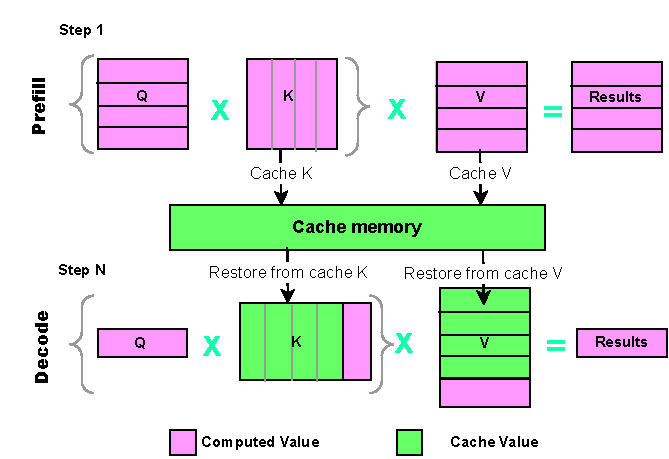
\includegraphics[scale=0.77]
 {KVCache.pdf}
\caption{KV Cache Mechanism showing the prefill stage with parallel processing and the decode stage with step-by-step generation. The KV cache stores key and value tensors during prefill for reuse during decoding.}
\label{fig:kv_cache_mechanism}
\end{figure}


As illustrated in Figure \ref{fig:kv_cache_mechanism}, the KV cache operates in two primary phases:
\begin{itemize}[leftmargin=*, topsep=1ex, partopsep=0pt, itemsep=0pt, parsep=0pt]
\item Prefill Stage: Executes the input prompt in parallel, computing and caching K/V pairs for all of the tokens in a single run.
\item Decode Stage: Produces tokens one at a time, calculating Q for the present token while retrieving cached K/V pairs for all past tokens.
\end{itemize}
This caching technique lowers computational expense by a spectacular amount, from O(n²) down to O(n) for each token, where n is the sequence length. Memory demands do increase linearly with sequence length, number of layers, and batch size, though, posing enormous challenges to servicing applications with lengthy contexts.
\subsection{Dynamic Memory Reclamation Strategies}
\label{sec:subsection}
Modern LLM serving systems employ a number of techniques for efficient management of KV cache memory:
\par CAKE (Cascading and Adaptive KV Cache Eviction) abstracts cache management as a "cake-slicing" problem, distributing memory to layers based on global attention patterns. CAKE resolves the memory redundancy by disentangling context and history, accelerating the inference without model retraining. The method distributes cache budgets dynamically based on importance scores derived from attention patterns, achieving significant memory reduction without model quality loss.
\par DynamicKV realizes task-aware adaptive KV cache compression by dynamically allocating budgets of retained tokens per layer based on task-specific attention patterns. Dynamic Budget Allocation and Progressive Cache Update are the two key steps in the method. It can retain model performance while only storing 1.7\% of the full KV cache, demonstrating outstanding efficiency for memory-constrained deployment.
\par LayerKV achieves serving latency optimization through layer-wise KV cache management. The system hierarchically allocates and manages KV blocks with intelligent prefetching and CPU-GPU collaboration to achieve low first-token time (TTFT) while making the best use of available memory resources.
\subsection{Memory and Hardware Constraints}
\label{sec:subsection}
The experiments for evaluation were run on NVIDIA A100-40G GPUs with paged-attention batching, block size 32, eager swap policy, and LRU eviction policy. The memory hierarchy is important for the performance of the system:

\begin{figure}[h]
\centering
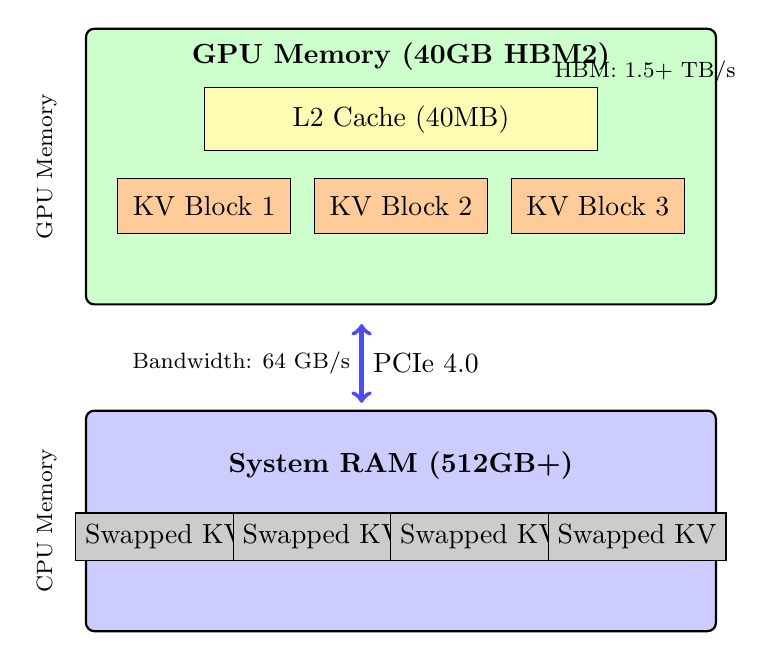
\begin{tikzpicture}[
    membox/.style={rectangle, draw, thick, rounded corners=3pt},
    kvblock/.style={rectangle, draw, fill=orange!40, minimum width=2.2cm, minimum height=0.7cm},
    cacheblock/.style={rectangle, draw, fill=yellow!30, minimum width=5cm, minimum height=0.8cm},
    swapblock/.style={rectangle, draw, fill=gray!40, minimum width=1.8cm, minimum height=0.6cm}
]
    % GPU Memory Container
    \node[membox, minimum width=8cm, minimum height=3.5cm, fill=green!20] (gpu) at (0,0) {};
    \node[font=\bfseries] at (0,1.4) {GPU Memory (40GB HBM2)};
    
    % L2 Cache inside GPU
    \node[cacheblock] (l2) at (0,0.6) {L2 Cache (40MB)};
    
    % KV Blocks in GPU (arranged in a row)
    \node[kvblock] (kv1) at (-2.5,-0.5) {KV Block 1};
    \node[kvblock] (kv2) at (0,-0.5) {KV Block 2};
    \node[kvblock] (kv3) at (2.5,-0.5) {KV Block 3};
    
  
   \node[font=\footnotesize] at (3.1,1.2) {HBM: 1.5+ TB/s};
    
    % PCIe Connection (bidirectional arrow)
    \draw[<->, ultra thick, blue!70] (-0.5,-2) -- node[right, black] {PCIe 4.0} node[left, black] {\footnotesize Bandwidth: 64 GB/s} (-0.5,-3);
    
    % System RAM Container
    \node[membox, minimum width=8cm, minimum height=2.8cm, fill=blue!20] (ram) at (0,-4.5) {};
    \node[font=\bfseries] at (0,-3.8) {System RAM (512GB+)};
    
    % Swapped KV blocks in RAM (arranged evenly)
    \node[swapblock] (swap1) at (-3,-4.7) {Swapped KV};
    \node[swapblock] (swap2) at (-1,-4.7) {Swapped KV};
    \node[swapblock] (swap3) at (1,-4.7) {Swapped KV};
    \node[swapblock] (swap4) at (3,-4.7) {Swapped KV};
    
    % Side annotations
    \node[rotate=90, anchor=center] at (-4.5,0) {\footnotesize GPU Memory};
    \node[rotate=90, anchor=center] at (-4.5,-4.5) {\footnotesize CPU Memory};
    
\end{tikzpicture}
\caption{Memory hierarchy in GPU-based LLM inference systems. The limited GPU memory (40GB) necessitates intelligent caching strategies and CPU-GPU coordination for handling large-scale concurrent requests.}
\label{fig:memory_hierarchy}
\end{figure}

As shown in Figure \ref{fig:memory_hierarchy}, the memory hierarchy presents several challenges:
\begin{itemize}[leftmargin=*, topsep=1ex, partopsep=0pt, itemsep=0pt, parsep=0pt]
\item GPU HBM: High bandwidth access (1.5+ TB/s) but low capacity (40-80GB).
\item System RAM: Offers larger capacity but requires PCIe transfers with significant latency.
\item Cache Architecture: Choice between shared and isolated caches significantly impacts performance in the presence of concurrent workloads.
\end{itemize}
Our tests showed that shared cache architectures suffer from around 40\% more latency and 25\% less throughput than isolated cache architectures when running in high concurrency conditions. This performance difference stresses the point of carefully analyzing and choosing suitable cache architectures when architecting systems for production environments. In particular, the latency increase and throughput reduction we saw in shared cache environments point to the requirement for careful architectural thought to be put into ensuring that systems are able to execute concurrent workloads effectively and reliably without sacrificing overall performance.
\subsection{Evaluation Metrics and Benchmarking}
\label{sec:subsection}
The performance analysis used five major indicators:
\par Time to First Token (TTFT): Measures latency from request submission to the creation of the first token. Results showed broad variability across datasets, with ShareGPT exhibiting latencies >24,000 ms as a result of longer prompt lengths.
\par Time per Output Token (TPOT): Calculates average generation time for each token. Experiments revealed that TPOT is very consistent within model families but varies significantly for different context lengths.
\par Memory Usage: Monitors GPU memory usage for inference. High cache allocations (320GB) cut latency by as much as 50\% for long-context datasets.
\par Goodput: It counts useful tokens received per second, taking into account cache evictions and recomputations.
\par Cache Hit Rate: Varies greatly from 0\% to 94.12\% depending on the characteristics of the workload and token reusability patterns.
\subsection{TokenSim Simulation Framework}
\label{sec:subsection}
TokenSim provides a flexible simulation framework for the investigation of KV cache policies decoupled from actual GPU resources. The platform consists of modular building blocks:
\begin{itemize}[leftmargin=*, topsep=1ex, partopsep=0pt, itemsep=0pt, parsep=0pt]
\item Scheduler: Handles token generation, timing, and queuing of requests.
\item Memory Manager: Provides cache allocation and eviction policies.
\item Model Interface: Mimics computational patterns of LLaMA2-7B, Mistral-7B, and InternLM2-7B.
\item Dataset Support: Contains BookCorpus, ShareGPT, LongBench, Needle-in-a-Haystack, and Wikipedia Structured datasets.
\end{itemize}
The simulator enables very controlled experiments using a large variety of cache sizes (40 – 320 GB), different eviction policies (both Least Recently Used (LRU) and Least Frequently Used (LFU) implementations), as well as a varying range of concurrency levels (from 2 to 10 concurrent sessions), hence enabling full and systematic testing of memory reclamation schemes.


\clearpage
\section {Related Work}
\subsection{Cache Compression and Layer Management
}
\label{sec:subsection}
\textbf{SqueezeAttention} \cite{wang2024squeezeattention2dmanagementkvcache} suggests 2D KV-cache management through layer-wise optimal budget allocation. The method computes cosine similarity between prompt representations before and after self-attention and applies K-Means clustering for layer grouping according to importance. More budgets are allocated to important layers while less influential layers undergo more aggressive compression. Top-k, Sliding Window, and Token Selection compression techniques are integrated into the method, achieving 70\% memory saving and 2.2× throughput improvement. Its sequence-wise eviction techniques, nevertheless, may potentially limit generalization, and clustering overhead reduces applicability in real-time environments.

\textbf{CAKE} \cite{qin2025cakecascadingadaptivekv} utilizes cascading and adaptive eviction and regards cache allocation as a "cake-slicing" issue. It quantifies the cache requirements of each layer while making a trade-off between attention spread and temporal evolution. CAKE adopts an eviction mechanism based on scores of both long-term significance and attention variance. CAKE minimizes KV cache consumption significantly with no loss in accuracy, and it obtains close-to-full memory performance using little cache. However, the cascading rationale and online attention analysis cause computational overhead, while the use of attention metrics might not be consistent with semantic significance.

\textbf{DynamicKV} \cite{zhou2025dynamickvtaskawareadaptivekv} introduces task-based adaptive compression that selects valuable tokens based on attention mechanisms across layers. The Top-K selection strategy keeps the most relevant tokens for each layer,
which supports layer-wise adaptive compression. The experiments demonstrate that it can maintain just 1. 7\% of the KV cache with slight quality degradation. However, the scarce computation budget influences accuracy, and generalization is still limited by the explored tasks and datasets.
\subsection{System-level Optimization Techniques
}
\label{sec:subsection}
\textbf{CAKE LayerKV} \cite{xiong2024layerkvoptimizinglargelanguage} addresses TTFT problems through layer-wise control and intelligent CPU-GPU coordination. The system tracks cache locations using mapping tables and calculates GPU retention based on free memory. It is trivially integrated with existing parallelization techniques while preventing PCIe contention through usage monitoring. LayerKV is simple, lightweight, and plug-compatible with existing systems , but may introduce TPOT without SLO-aware scheduling.

\textbf{CacheGen} \cite{cachegencitation} optimizes KV cache sharing across distributed systems through adaptive compression using delta encoding, quantization, and arithmetic coding. It dynamically adjusts compression to meet SLOs under varying network conditions, achieving 3.7× faster response and 4.3× lower transmission costs. While providing plug-and-play compatibility, its effectiveness depends on high context reuse, limiting its applicability in dynamic scenarios.

\textbf{InstAttention} \cite{10946721} offloads attention computation to computational storage drives (CSDs), utilizing internal bandwidth to avoid PCIe bottlenecks. The flash-aware attention mechanism and SparF algorithm reduce computation and KV cache requirements without compromising accuracy. However, the compute-in-storage architecture requires specialized hardware and shows limited benefits when SSDs connect through PCIe switches.

\subsection{Token-level Eviction Strategies}
\label{sec:subsection}
\textbf{H2O} \cite{ssdcitation} selects "heavy hitter" tokens by computing a cumulative attention score for each token and frames eviction as an optimization problem trading off token importance against recency. By retaining only those tokens with the largest impact, H2O drastically reduces the overall cache footprint with no effect on model performance. However, because its selection process depends on variance in attention scores, H2O might perform inadequately on tasks where attention is focused relatively uniformly over all tokens.

\textbf{Crowd} \cite{10735473} adopts a neighborhood‐based eviction policy, where attention scores are averaged over sliding windows to determine the local relevance of each token. In this policy, tokens with the lowest window average attention are evicted, whereas context‐critical tokens are retained. The success of this approach depends upon the selection of the window size, and it typically needs dataset‐specific tuning to achieve the appropriate balance between eviction aggressiveness and contextual fidelity.

\textbf{WeightedKV} \cite{10889583} employs an asymmetric compression scheme in which keys associated with lower attention weights are evicted, and the remaining value vectors are merged according to their weighted attention scores. This training‐free approach conserves more information than symmetric eviction methods and delivers superior performance on longer input sequences. The one trade‐off is that the merged value representations cannot be undone, which limits flexibility for any downstream adaptation or post‐processing.
\subsection{Alternative Approaches}
\label{sec:subsection}
\textbf{Activation Sequence Caching (ASC)} \cite{10.1145/3656019.3676945} stores intermediate activation outputs rather than the usual key–value tensor pairs, trading off extra memory use and additional data‐transfer overhead to perform the required computations. In single‐GPU benchmarks, this approach achieves a remarkable 78.3\% speedup over FlexGen, making it highly effective in environments where memory is the primary constraint. However, on GPUs with lower computational throughput, the overhead of those extra computations can erode performance gains, so ASC may not deliver the same benefits in all hardware settings.

\textbf{HCache} \cite{10.1145/3689031.3696072}, by contrast, targets multi‐turn dialogue workloads: it persists hidden‐state representations across consecutive requests instead of fully rebuilding the KV cache each time. This design minimizes both computation and I/O compared to complete KV restoration, allowing it to slot neatly into existing inference pipelines. On the downside, HCache requires tuning that is specific to the underlying hardware, and its performance characteristics may not transfer seamlessly across different GPU architectures.

Together, they represent the spectrum of KV cache optimization techniques—each making different trade‐offs among memory efficiency, computation overhead, and system complexity. Our end‐to‐end evaluation using TokenSim provides a uniform, holistic view of how those trade‐offs unfold under realistic serving workloads, enabling informed choice regarding which caching strategy best fits a given deployment environment.
\clearpage
\section {Methodology}

\subsection{Virtual Machine Platform}
\label{sec:subsection}
Table \ref{tab:vm_config} shows the virtual machine environment configuration we used for this experiment, including five machines. 
 \vspace{-5pt}
\begin{table}[H]
\centering
\caption{VM Environment Configuration}
\label{tab:vm_config}
\begin{tabular}{@{}l|p{0.12\columnwidth}p{0.12\columnwidth}p{0.12\columnwidth}p{0.12\columnwidth}p{0.12\columnwidth}@{}}
\toprule
\textbf{Property} & \textbf{1} & \textbf{2} & \textbf{3} & \textbf{4} & \textbf{5}     \\
\midrule
OS & Fedora 40&Ubuntu 24.0.2&Ubuntu 24.0.2 &Ubuntu 24.04.2&Ubuntu 24.04.2  \\
VirtualBox & Yes & Yes & Yes & Yes & Yes  \\
RAM (GB)& 6 & 4 & 8 & 8 & 8   \\
HDD Space  & 80 & 100  & 100 & 100& 100   \\
vCPUs & 4 & 6 & 6 & 16 & 6   \\
Packages  & git 2.49.0 & git 2.43.0 & git 2.43.0 & git 2.43.0 & git 2.43.0  \\
  & conda 24.9.1 & conda 24.9.2 & conda 24.9.2& conda 24.9.2& conda 24.9.2  \\
  & VIM 9.1 & VSCode 1.101.1  & VSCode 1.101.0 & VSCode 1.101.0& VSCode 1.101.0 \\
\bottomrule
\end{tabular}
\end{table}


\vspace{-1em}
\subsection{Simulation}
\label{sec:subsection}
 We evaluate the performance of a large language model (LLM) inference system using the TokenSim simulation framework. The main purpose of TokenSim is to simulate both hardware and software settings without needing a real GPU. It helps researchers test how models behave with different memory and scheduling settings. TokenSim includes a scheduler that controls when and how tokens are generated. It has a memory manager that keeps track of how memory is used and when items are removed from the cache. The simulator is modular, so different parts like the scheduler, cache, and model can be changed or improved easily. Researchers can measure how different factors affect performance with various datasets and models. This makes TokenSim a useful tool for improving the memory efficiency of LLMs.
\subsection{Models}
\label{sec:subsection}
We select three representative models to analyze how different model architectures interact with various cache configurations and strategies, providing a foundation for performance evaluation.

LLaMA-2 7B \cite{touvron2023llama2}is a 32-layer Transformer model with 4096-dimensional hidden states and 32 attention heads. It integrates rotary positional embeddings and grouped-query attention to improve inference efficiency. With its versatile architecture, LLaMA-2 supports a wide range of tasks such as text generation, code completion, summarization, and interactive chatbot applications. The model relies heavily on KV caching for fast, autoregressive decoding, making it well-suited for handling long input sequences with reduced computational overhead.  

Mistral 7B \cite{mistral2023} offers an architecture similar in scale to LLaMA-2 but incorporates a sliding window attention mechanism alongside grouped-query attention. This design improves memory efficiency, particularly in constrained or latency-sensitive environments. Mistral is optimized for real-time dialogue, instruction-following, and on-device use. Its KV cache behavior is relevant for evaluating token-level reuse, eviction, and compact cache strategies due to the nature of its windowed attention. 

InternLM2 7B \cite{internlm2}is a Transformer model fine-tuned for multi-turn dialogue and potentially multimodal tasks. It excels in scenarios requiring long-term memory and contextual coherence, such as multi-turn Q\&A, structured reasoning, and dialogue systems. InternLM2 supports advanced cache optimization techniques, including KV compression, streaming, and offloading, making it a strong candidate for research into dynamic cache management strategies.  
 
\subsection{Datasets}
\label{sec:subsection}
We also select five datasets that represent diverse use cases to evaluate how language models interact with the KV cache under different input characteristics.

LongBench v2 contains tasks that require understanding and working with very long inputs. It is designed to measure how language models handle tasks like summarizing documents or answering detailed questions \cite{longbenchv2}. This helps test how well a model uses and maintains cached information over long input spans.

Needle-in-a-Haystack is a benchmark where the model needs to pick out rare or hidden items from long text. It checks if the model can remember small but important parts of earlier content \cite{needle}. This is helpful for cache testing because it shows whether the memory system keeps key details or loses them too soon.

ShareGPT includes a large number of user-created chat conversations collected from an open API. It is used to train or test models on back-and-forth dialogue across multiple turns \cite{sharegpt}. Since conversation history can be reused, this dataset is useful for seeing how cache memory is reused or overwritten across turns.

BookCorpus is made up of long-form stories and books written by unknown authors and shared freely. It’s often used to teach models how to understand and generate continuous, natural text \cite{bookcorpus}. This dataset supports KV cache experiments where older tokens may still matter after many paragraphs.

Wikipedia Structured Contents includes data from Wikipedia that’s been turned into structured files, like organized lists or records. It’s useful for checking how models deal with facts and structured information \cite{wikidata}. This kind of dataset shows how caching can help or hurt when the model needs to remember factual details over long sections.
 

\subsection{Evaluation Metrics}
\label{sec:subsection}
Table \ref{tab:evaluation_metrics} illustrates the evaluation metrics we used in the experiment and how to measure them.
\begin{table} [H]
\small
\centering
\caption{Evaluation Metrics}
\vspace{-1 em}
\label{tab:evaluation_metrics}
\begin{tabular}{@{}p{0.26\columnwidth} p{0.68\columnwidth}@{}}
\toprule
\textbf{Metric} & \textbf{Formula or Measurement} \\
\midrule
Time to First Token (TTFT) & Measured via median latency \texttt{prompt\_time.p50} (sec). \\
Time per Output Token (TPOT) & 
\makebox[0pt][l]{\(\displaystyle \text{TPOT} = \frac{1000}{\text{output\_token\_ps}} \quad \text{(ms/token)}\)} \\
Memory Usage & Measured by tracking GPU memory before and after inference (GB). \\
Goodput & Measured via \texttt{output\_token\_ps} (tokens/sec). \\
Eviction Rate & 
\makebox[0pt][l]{\(\displaystyle \text{Eviction Rate} = \frac{\#\text{Evicted Entries}}{\#\text{Inserted Entries}} \times 100\% \)} \\
\bottomrule
\end{tabular}
\end{table}

\section {Evaluation}
This section presents our evaluation of dynamic memory reclamation techniques in large language models (LLMs). We tested three 7B-parameter models—LLaMA2 \cite{touvron2023llama2}, Mistral \cite{mistral2023}, and InternLM2  \cite{internlm2} —on five benchmark datasets. The evaluation focuses on how cache size, session concurrency, token length, and system architecture impact performance. Metrics include p99 latency, throughput, cache hit rate, and stage-wise latency breakdown. The experiments were conducted using a simulation framework modeled after TokenSim, ensuring reproducibility and consistency. 
\subsection{How Cache Size Affects Latency}
We started by testing how increasing the cache size impacts prompt latency. As shown in Figure \ref{fig1}, larger caches help reduce latency across all datasets, but the effect is especially strong for ShareGPT \cite{sharegpt} and LongBench2 \cite{longbenchv2}, which use longer prompts. That’s because longer contexts benefit more from reusing cached key-value pairs.
LLaMA2 \cite{touvron2023llama2} consistently showed the lowest latency, especially as the cache size increased. This shows that the model can take full advantage of the extra memory to reduce processing delays.
\begin{figure}[H]
    \centering
    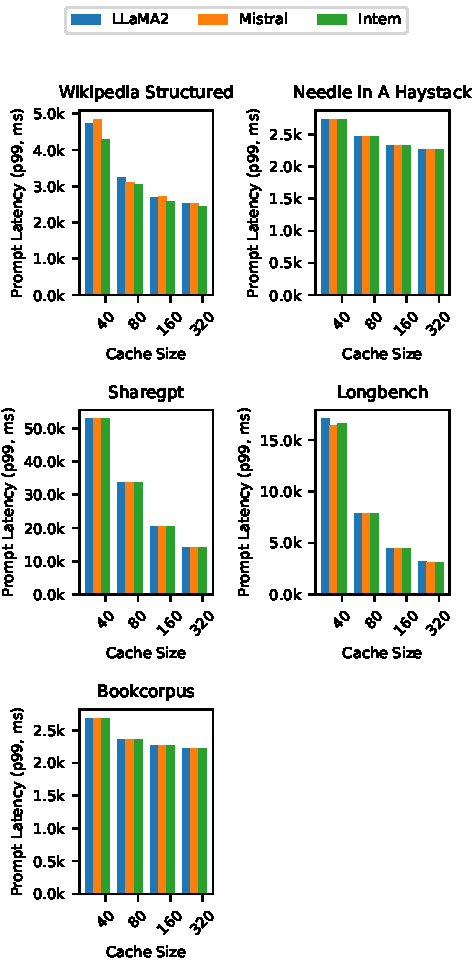
\includegraphics[scale=0.75]{figure1_combined_latency.pdf}
    \caption{Prompt latency (p99, in milliseconds) across different cache sizes for five datasets.}
    \label{fig1}
\end{figure}
\subsection{Eviction Policies: LRU vs. LFU}
Effective cache eviction is essential for maintaining low latency and high throughput, especially when memory is limited. In this subsection, we compare two commonly used policies: Least Recently Used (LRU) and Least Frequently Used (LFU). Although both aim to remove the least useful entries from the KV cache, their behavior diverges significantly under different workloads.

Figure \ref{fig:3} illustrates cache hit rates across five datasets under LRU and LFU policies at various cache sizes. While both policies yield similar hit rates at larger cache sizes, LFU consistently outperforms LRU in smaller memory settings, particularly for datasets with recurring token patterns, such as ShareGPT and LongBench. This is because LFU retains frequently reused tokens even across session boundaries, while LRU may evict them too early.
\begin{figure}[htbp]
    \centering

    \begin{subfigure}[b]{0.47\columnwidth}
        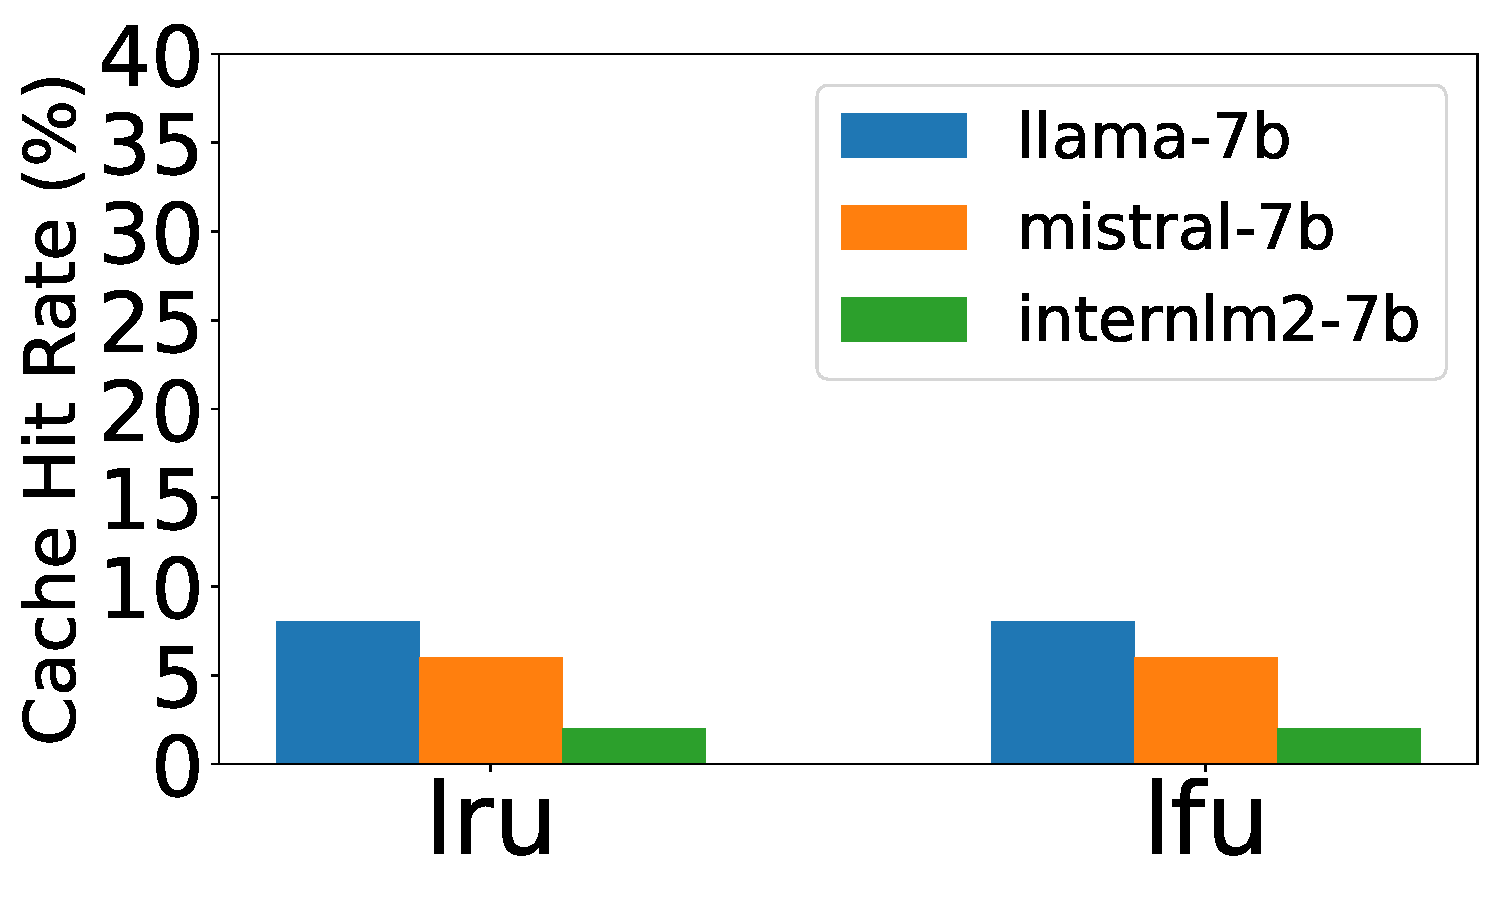
\includegraphics[width=\linewidth]{figure3and4/sharegpt_cache_hit_rate_vs_eviction.pdf}
        \caption{ShareGPT}
    \end{subfigure}
    \hfill
    \begin{subfigure}[b]{0.47\columnwidth}
        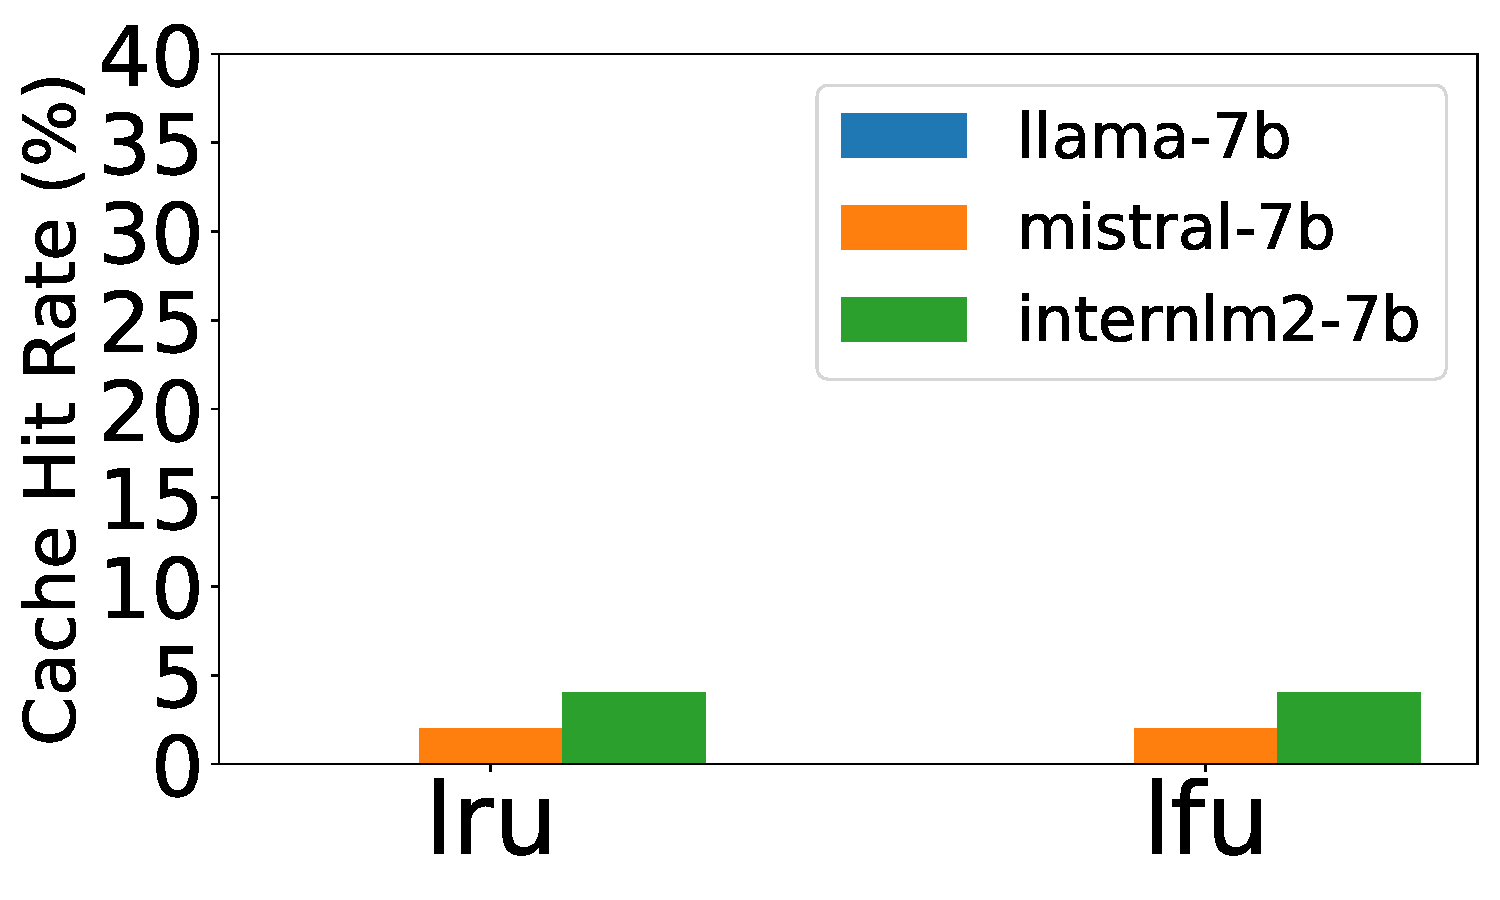
\includegraphics[width=\linewidth]{figure3and4/bookcorpus_cache_hit_rate_vs_eviction.pdf}
        \caption{BookCorpus}
    \end{subfigure}

    

    \begin{subfigure}[b]{0.47\columnwidth}
        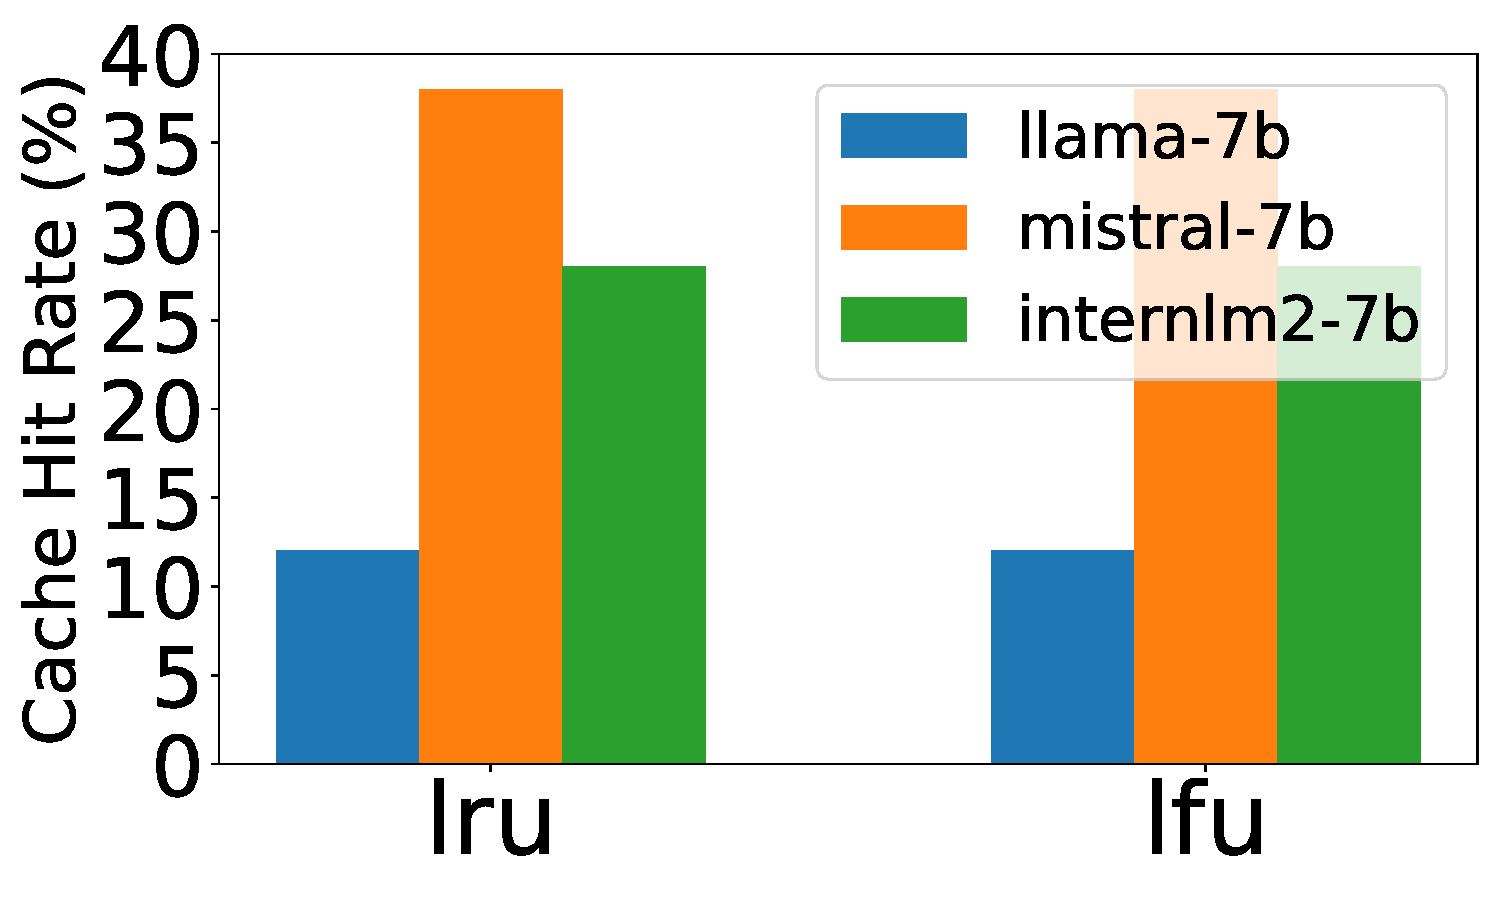
\includegraphics[width=\linewidth]{figure3and4/needle_in_a_haystack_cache_hit_rate_vs_eviction.pdf}
        \caption{Needle-in-a-Haystack}
    \end{subfigure}
    \hfill
    \begin{subfigure}[b]{0.47\columnwidth}
        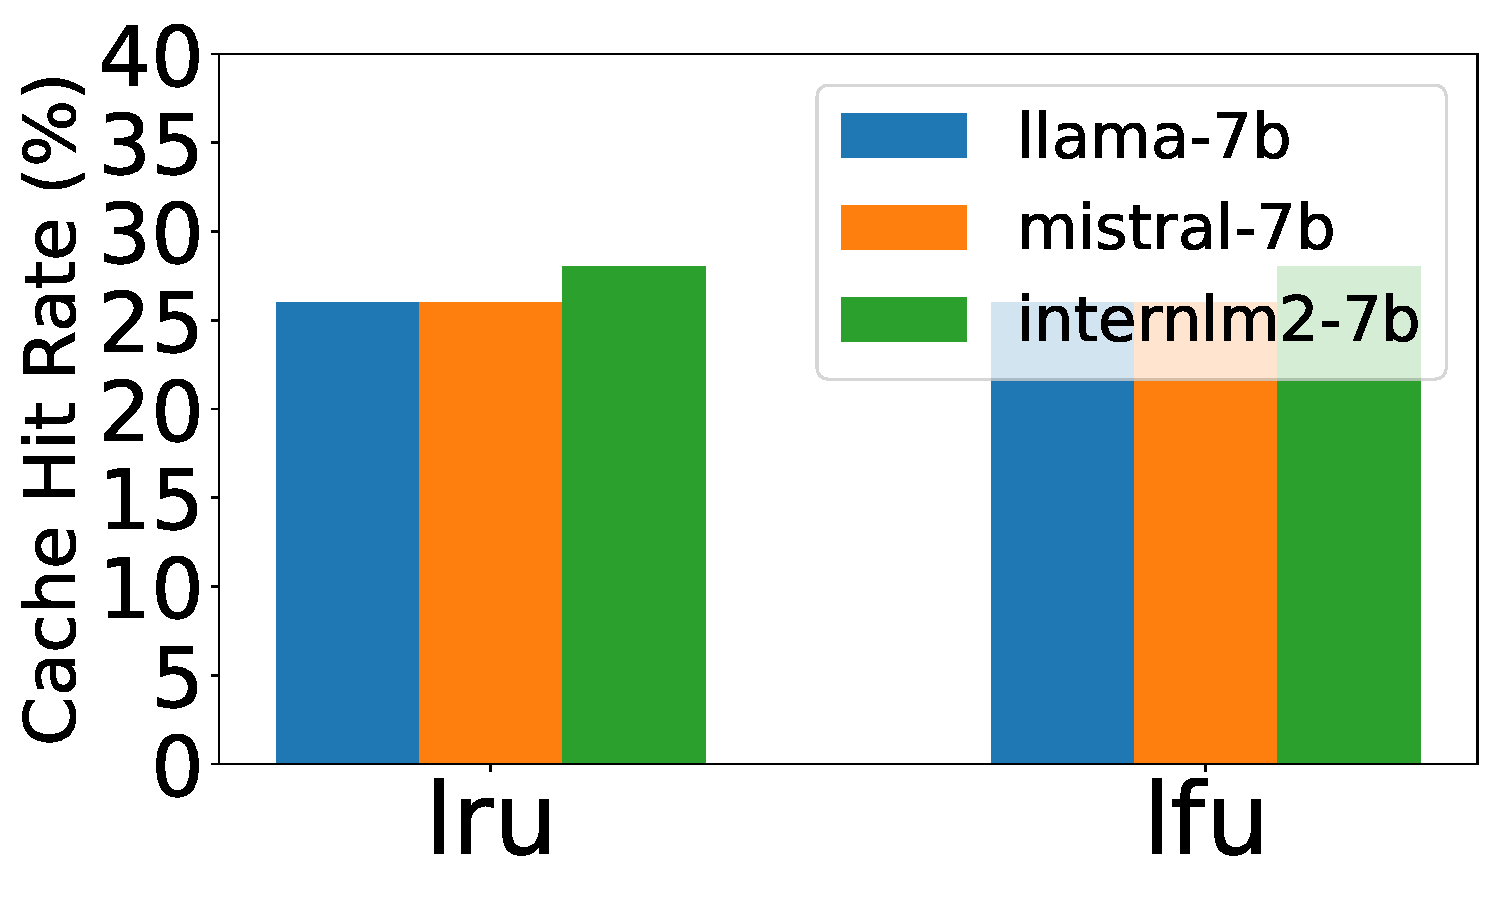
\includegraphics[width=\linewidth]{figure3and4/longbench_cache_hit_rate_vs_eviction.pdf}
        \caption{LongBench}
    \end{subfigure}

    \vspace{0.5em}

    \begin{subfigure}[b]{0.47\columnwidth}
        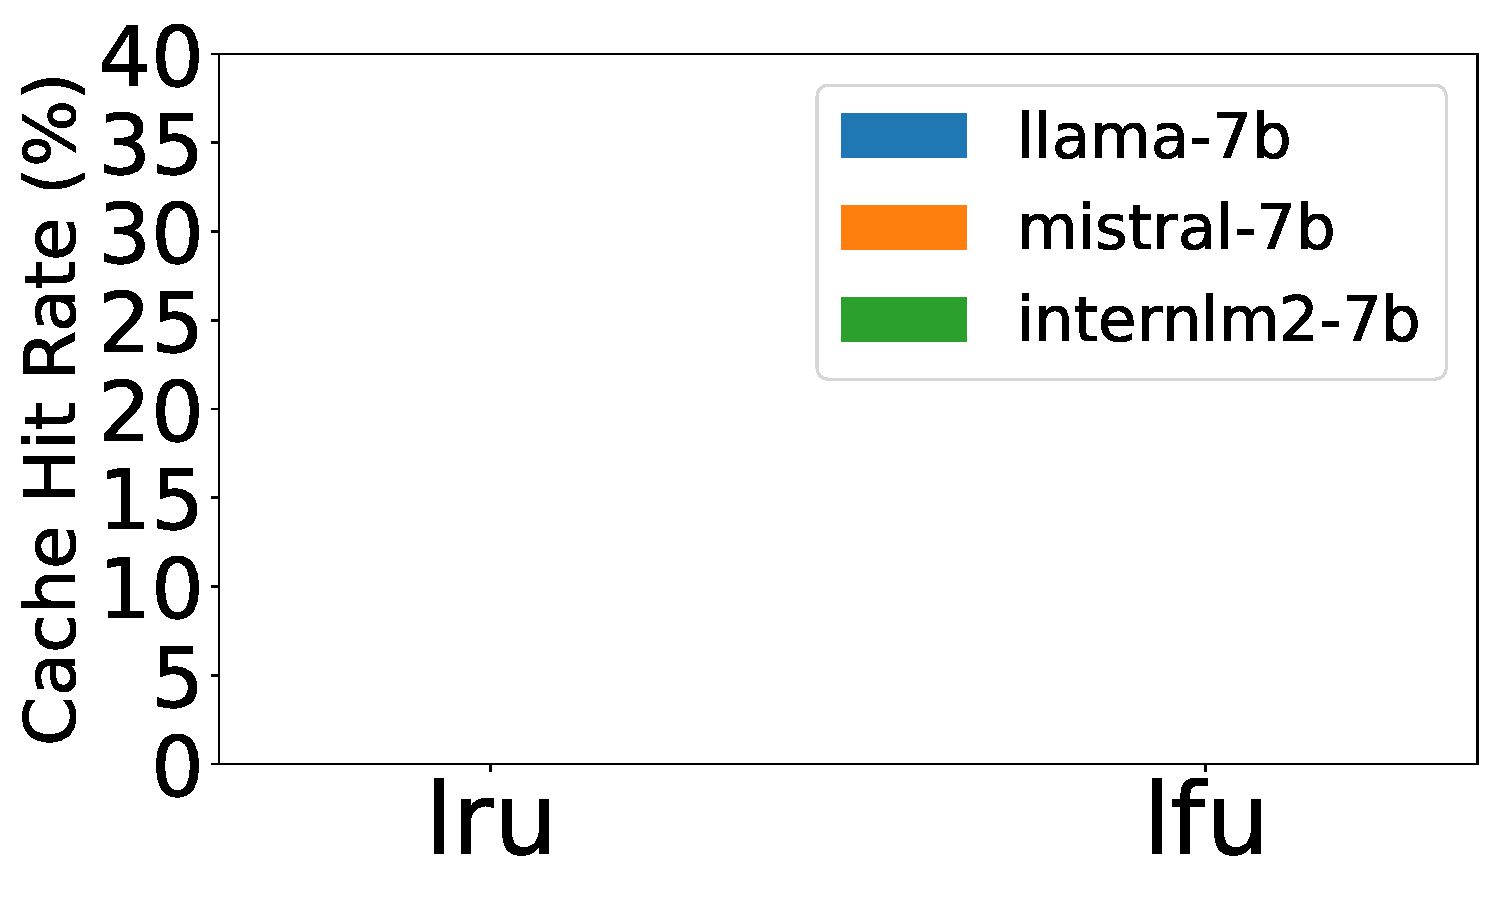
\includegraphics[width=\linewidth]{figure3and4/wikipedia_structured_cache_hit_rate_vs_eviction.pdf}
        \caption{Wikipedia Structured}
    \end{subfigure}

    \caption{Eviction Policy vs. Cache Hit Rate.}
    \label{fig:3}
\end{figure}\par However, hit rate alone doesn't always reflect real-world performance differences. To better understand the practical latency impact of eviction strategies, we analyzed the token generation time (in milliseconds) under both policies across multiple datasets and models. LFU consistently yields lower generation time in long-context datasets like LongBench and ShareGPT, where frequently accessed tokens benefit from LFU’s reuse-aware strategy. In contrast, LRU shows similar or slightly better performance in shorter-context datasets like Wikipedia and Needle, likely due to its simpler access pattern and lower overhead. These findings suggest that LFU is better suited for memory-constrained, long-sequence workloads, while LRU may be sufficient or even preferable for shorter prompts where cache pressure is minimal.


\subsection{System Behavior with More Sessions}
Next, we evaluated how the models perform under growing concurrency, simulating multiple simultaneous inference sessions. We varied the number of sessions from 2 to 10 and measured both latency and throughput.
As shown in Figure \ref{fig7a}, latency increases gradually at lower concurrency levels but spikes after 8 sessions, especially for InternLM2 and Mistral. LLaMA2 scaled more gracefully, maintaining lower latency at higher session counts. This indicates that LLaMA2 is better optimized for multi-session environments, possibly due to more efficient GPU memory usage and parallelism.
\begin{figure}[h]
    \centering
    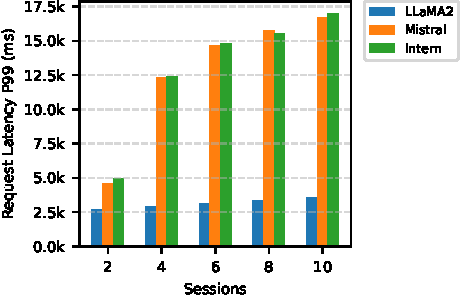
\includegraphics[scale=0.8]{figure7a.pdf}
    \vspace{-1.0em}  
    \caption{Request Latency across different models at varying session counts (QPS).}
    \label{fig7a}
\end{figure}
\par To complement latency findings, we plotted throughput across datasets in Figure \ref{fig8b}. ShareGPT consistently achieved the highest throughput regardless of session count, likely due to high cache reuse in long sequences. Needle-in-a-Haystack had the lowest throughput, reflecting its frequent context switching and shorter prompts, which reduce cache utility.

The architectural choice of shared vs. isolated cache also played a role. In shared cache settings, models had to coordinate access and eviction across sessions, leading to contention. Isolated caches eliminated this overhead but increased memory usage. These trade-offs become more apparent as concurrency rises.
\begin{figure}[h]
    \centering
    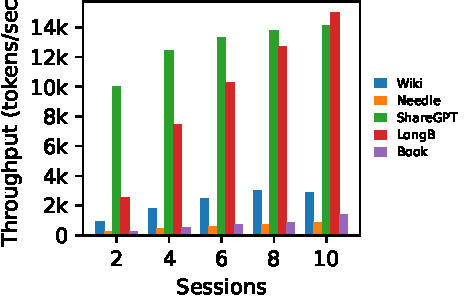
\includegraphics[scale=0.8]{figure8b.pdf}
    \vspace{-1.0em}  
    \caption{Throughput (in tokens/sec) across different datasets at varying session counts (QPS).}
    \label{fig8b}
\end{figure}
\par During these tests, we observed different system bottlenecks depending on the model and scenario. These are summarized in Table \ref{tab:bottleneck}. For instance, LLaMA2 reached GPU memory limits at high QPS, whereas InternLM2 encountered paging overhead in shared cache setups.
\begin{table}[h]
\renewcommand{\arraystretch}{0.95}  % Reduce row height
\small  % Shrink font (can revert to \small if needed)
\centering
\caption{System Bottlenecks Based on Observed Scalability Limits}
\rowcolors{2}{gray!10}{white} % Start coloring from the second row
\vspace{-0.5em}
\begin{tabularx}{\linewidth}{l p{2.5cm} X}
\hline
\textbf{Model} & \textbf{Scenario} & \textbf{Observed Bottleneck} \\
\hline
LLaMA2-7B & High QPS, 512 tokens & GPU memory pressure due to limited KV cache \\
\hline
Mistral-7B & 8192 tokens & Increased latency from cache evictions at large lengths \\
\hline
InternLM2-7B & Shared cache, QPS 10 & Communication overhead due to paging and coordination \\
\hline
\end{tabularx}

\label{tab:bottleneck}
\end{table}
\subsection{Token Length Sensitivity}
Token length is another critical factor influencing LLM performance. As more tokens are processed in a single session, the cache grows, and memory pressure builds. We varied the number of tokens per session from 512 to 16384 and observed the impact on latency, throughput, and cache hit rate.

Figure \ref{fig9} shows that latency is relatively stable up to about 4096 tokens. Beyond that, latency increases sharply for all three models, with a dramatic rise after 8192 tokens. This indicates that the cache is saturated, and recomputation of evicted tokens becomes more frequent, leading to delays..
\begin{figure} [h]
    \centering
   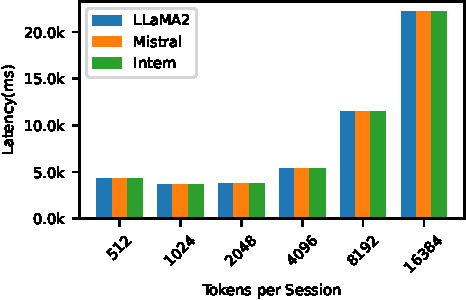
\includegraphics[scale=0.8]{figure9_latency_vs_tokens.pdf}
    \vspace{-1.0em}
    \caption{Latency (in milliseconds) versus Tokens per Session for three models: LLaMA2, Mistral, and Intern.}
    \vspace{-1.0em}  
    \label{fig9}
\end{figure}
\par In Figure \ref{fig12} reinforces this finding by showing cumulative p99 latency across QPS levels. LLaMA2 again outperformed the others, staying within tolerable latency limits even at higher loads. InternLM2 and Mistral both exhibited steep latency increases beyond QPS 6, suggesting that their internal cache management mechanisms are less efficient at scale.
\begin{figure} [h]
    \centering
   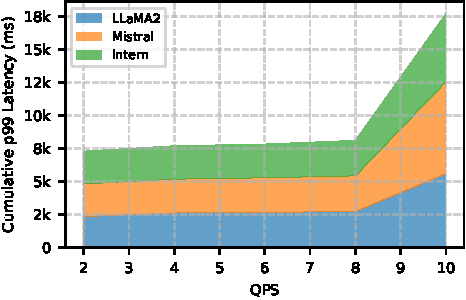
\includegraphics[scale=0.8]{figure12_latency_vs_model_stacked.pdf}
   \vspace{-1.0em}  
    \caption{Model Scalability Comparison: Stacked area chart of cumulative p99 latency (ms) across increasing QPS values for LLaMA2, Mistral, and Intern models.}
    \vspace{-1.0em}  
    \label{fig12}
\end{figure}
\par Cache hit rate also improved with longer token lengths, as shown in Figure \ref{fig11}. With short inputs (512 tokens), there’s minimal reuse, resulting in a 0\% hit rate. At 8192 and beyond, the hit rate stabilized at over 94\% across all models. This suggests that while long prompts stress the cache, they also offer better opportunities for reuse if memory is sufficient.

These results support the idea of dynamically adjusting cache size or applying smarter eviction policies for long sessions to sustain performance.
\begin{figure}
    \centering
   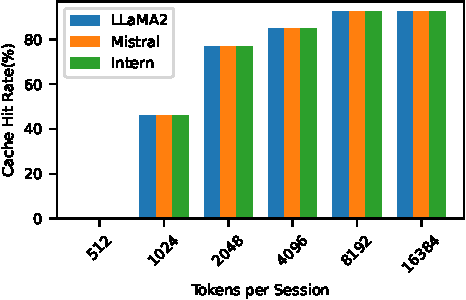
\includegraphics[scale=0.8]{figure11_cache_hit_vs_tokens.pdf}
    \vspace{-1.0em}
    \caption{Cache Hit Rate (\%) versus Tokens per Session for LLaMA2, Mistral, and Intern models.}
    \label{fig11}
\end{figure}
\subsection{Where the Time Goes: Latency Breakdown}
To understand where time is being spent during inference, we broke down latency into four key stages: preprocessing, inference, cache access, and postprocessing. This helps identify performance bottlenecks beyond just the total prompt latency or throughput.

As shown in Figure \ref{figure13}, the inference stage is by far the largest contributor to overall latency, accounting for nearly 80\% of the total time across all datasets. Cache access comes next, averaging around 8\%, followed by postprocessing. Preprocessing time remains negligible in nearly all workloads.
\begin{figure}[H]
    \centering
   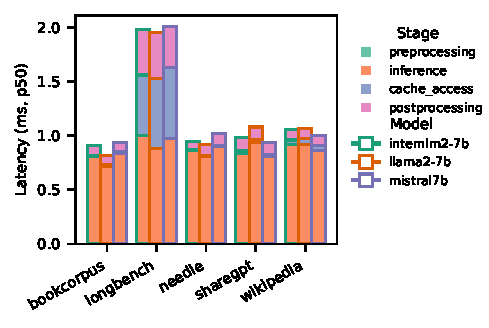
\includegraphics[scale=0.9]{figure13.pdf}
    \caption{Stacked‐bar chart showing the latency breakdown across the four processing stages for each dataset–model pair.}
    \label{figure13}
\end{figure}
\par Looking across datasets in Figure \ref{figure16}, we find that LongBench has the highest cache access and postprocessing latency, due to its long sequences and structured outputs. Datasets like Bookcorpus and Wikipedia show consistently low latency in all stages, indicating lower computational and memory overhead.
 \begin{figure}[H]
    \centering
   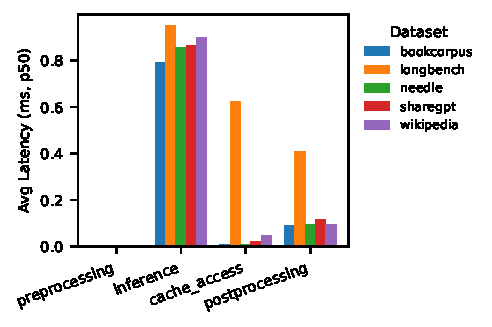
\includegraphics[scale=0.9]{figure16.pdf}
    \vspace{-1.0em}
    \caption{Dataset‐wise average latency per stage, showing how the relative cost of cache access and postprocessing varies across workloads }
    \label{figure16}
\end{figure}
\vspace{-1.0em}
To further analyze the cache behavior, we examined how long it takes to access cached values versus recomputing them when evicted. These results are summarized in Table \ref{tab:15}. For short-sequence datasets such as Bookcorpus and Needle, cache access latency is minimal, often under 0.03 ms. This suggests that the cache performs efficiently when workloads are light and token reuse is low. However, for long-sequence datasets like LongBench and ShareGPT, cache access latency spikes significantly when recomputation is triggered, reaching up to 7.50 ms. These workloads tend to fill up the cache quickly, leading to more frequent evictions and recomputations. This shows that when cache eviction occurs, the recomputation penalty is non-trivial, especially under constrained memory or high-concurrency conditions. Consequently, optimizing eviction strategies and cache sizing becomes increasingly important in long-context scenarios to avoid latency spikes that could degrade user experience.
\begin{table}[ht]
  \centering
  \small
  \setlength{\tabcolsep}{3pt}
  \caption{Cache‐access latency during retrieval vs.\ recomputation, reporting both median and maximum values.}
  \label{tab:15}
  \begin{tabular}{
    >{\columncolor{gray!20}}l
    >{\columncolor{gray!20}}l
    >{\columncolor{gray!20}}c
    >{\columncolor{gray!20}}c
  }
    \toprule
    Dataset 
      & Model 
      & \makecell{Cache P50\\(ms)}
      & \makecell{Cache Max\\(ms)} \\
    \midrule
    bookcorpus & internlm2-7b & 0.01 & 0.03 \\
    bookcorpus & llama2-7b    & 0.01 & 0.10 \\
    bookcorpus & mistral7b    & 0.01 & 0.03 \\
    longbench  & internlm2-7b & 0.56 & 6.36 \\
    longbench  & llama2-7b    & 0.65 & 7.50 \\
    longbench  & mistral7b    & 0.66 & 6.83 \\
    needle     & internlm2-7b & 0.01 & 0.10 \\
    needle     & llama2-7b    & 0.01 & 0.09 \\
    needle     & mistral7b    & 0.01 & 0.08 \\
    sharegpt   & internlm2-7b & 0.02 & 0.42 \\
    sharegpt   & llama2-7b    & 0.02 & 0.36 \\
    sharegpt   & mistral7b    & 0.02 & 0.41 \\
    wikipedia  & internlm2-7b & 0.04 & 0.14 \\
    wikipedia  & llama2-7b    & 0.05 & 0.17 \\
    wikipedia  & mistral7b    & 0.05 & 0.22 \\
    \bottomrule
  \end{tabular}
\end{table}
 
\section {Discussion}

Our evaluation shows that KV (Key-Value) cache configuration significantly affects large language model (LLM) inference performance. Increasing cache size consistently improves p99 latency and throughput, especially on long-context datasets like ShareGPT and LongBench, where latency drops by up to 50\% and throughput increases by over 10,000 tokens per second. These gains result from storing more key-value pairs in memory, reducing the need to recompute attention over long token histories, and enabling more efficient generation.

Our exploration of cache replacement strategies reveals important trade-offs. Although commonly used algorithms such as Least Recently Used (LRU) and Least Frequently Used (LFU) show comparable average hit rates across many settings, their effectiveness varies drastically depending on the specific dataset and context length, with hit rates ranging from 0\% to as high as 94.12\%. Despite these variations, the overall impact of the replacement strategy on average token generation time remains limited, indicating that other factors—such as the efficiency of inference computation—may dominate in most scenarios.

We also evaluate the scalability of two cache management architectures: shared and isolated. In scenarios with low concurrency (i.e., fewer parallel inference sessions), both approaches deliver similar performance. However, as the number of concurrent sessions increases, shared cache architectures consistently outperform isolated ones in terms of throughput. Notably, LLaMA2-7B demonstrates the best scalability characteristics, maintaining high throughput across all session configurations when using shared caches. This suggests that shared cache models can leverage temporal and spatial locality across sessions more effectively under high concurrency, though they may face challenges related to contention and cache eviction under extreme loads.

A latency breakdown analysis further clarifies the performance landscape. The inference phase, where the model computes attention and generates outputs, remains the dominant bottleneck, accounting for approximately 80\% of total end-to-end latency. Cache access time typically contributes around 8\%, but in complex settings—particularly those with deep context windows such as LongBench—the cache access overhead can rise significantly, at times exceeding 30\% of total latency. This highlights the need to optimize both memory access patterns and model computation.
Certainly. Here’s a shortened version of the last two paragraphs:

Based on our findings, we recommend using larger KV caches for long-context tasks to reduce recomputation and improve reuse. Shared cache architectures scale better under high concurrency, offering higher throughput. Since inference remains the primary bottleneck, further optimizations should focus on model computation, such as quantization, operator fusion, and hardware-aware scheduling.

Future work can explore adaptive cache policies that adjust to workload changes in real time. Smarter replacement strategies that consider session importance and access patterns may improve cache efficiency. Hybrid architectures—combining shared and isolated modes or adding fast secondary storage like NVMe—also hold promise for scaling LLM inference in dynamic environments.


\section {Conclusion}
 This study comprehensively evaluated the performance of large language model (LLM) inference systems using TokenSim, a simulation framework designed to model scheduling and memory behavior. Controlled experiments were conducted across three major areas: memory cache configurations, scalability, and latency breakdown analysis. The ablation study varied cache sizes (40GB, 80GB, 160GB, 320GB), eviction policies (e.g., LRU, LFU), and cache architectures (shared vs. isolated) to assess their impact on system throughput, latency, and cache hit rate. Results indicated that smaller caches and shared architectures under concurrent workloads led to significant performance degradation, while isolated caches offered more stable behavior. Scalability experiments showed that as the number of sessions and tokens per session increased, latency rose steadily and throughput gains diminished beyond a saturation threshold, exposing system bottlenecks. To further identify latency contributors, TokenSim’s event-driven infrastructure was instrumented with fine-grained timestamps across four stages: preprocessing, inference, cache access, and postprocessing. The analysis confirmed that inference consistently dominated latency, with cache access as a secondary bottleneck, especially under shared cache mode. Figures and tables illustrated both absolute and relative latency patterns across datasets and models. Based on these findings, several enhancements tailored to TokenSim are proposed: incorporating dynamic cache partitioning within the shared cache manager, simulating hybrid RAM–NVMe cache tiers, and implementing load-aware adaptive inference scheduling using SimPy. Extending the simulator to model distributed caching and hardware-aware acceleration could also offer valuable insights into real-world deployments and further improve the system’s responsiveness under scale. Future work may include support for distributed cache architectures and hardware-aware inference acceleration, offering deeper insights into real-world LLM system behavior under scale.
 


 

%%
%% The acknowledgments section is defined using the "acks" environment
%% (and NOT an unnumbered section). This ensures the proper
%% identification of the section in the article metadata, and the
%% consistent spelling of the heading.
 

%%
%% The next two lines define the bibliography style to be used, and
%% the bibliography file.
\clearpage
\makeatletter
\global\let\@balance@postpone\relax
\global\let\@balancedfalse\relax
\global\let\balance\relax
\makeatother
 
\bibliographystyle{ACM-Reference-Format}
\bibliography{BibTeX}




%%
%% If your work has an appendix, this is the place to put it.
\clearpage
\appendix
\twocolumn[ % Fake single-column for the figure
\section{Screenshot of GitHub repository which shows LaTeX Source Folder}
\vspace{-2em}
\begin{figure*}[t!]
    \centering
    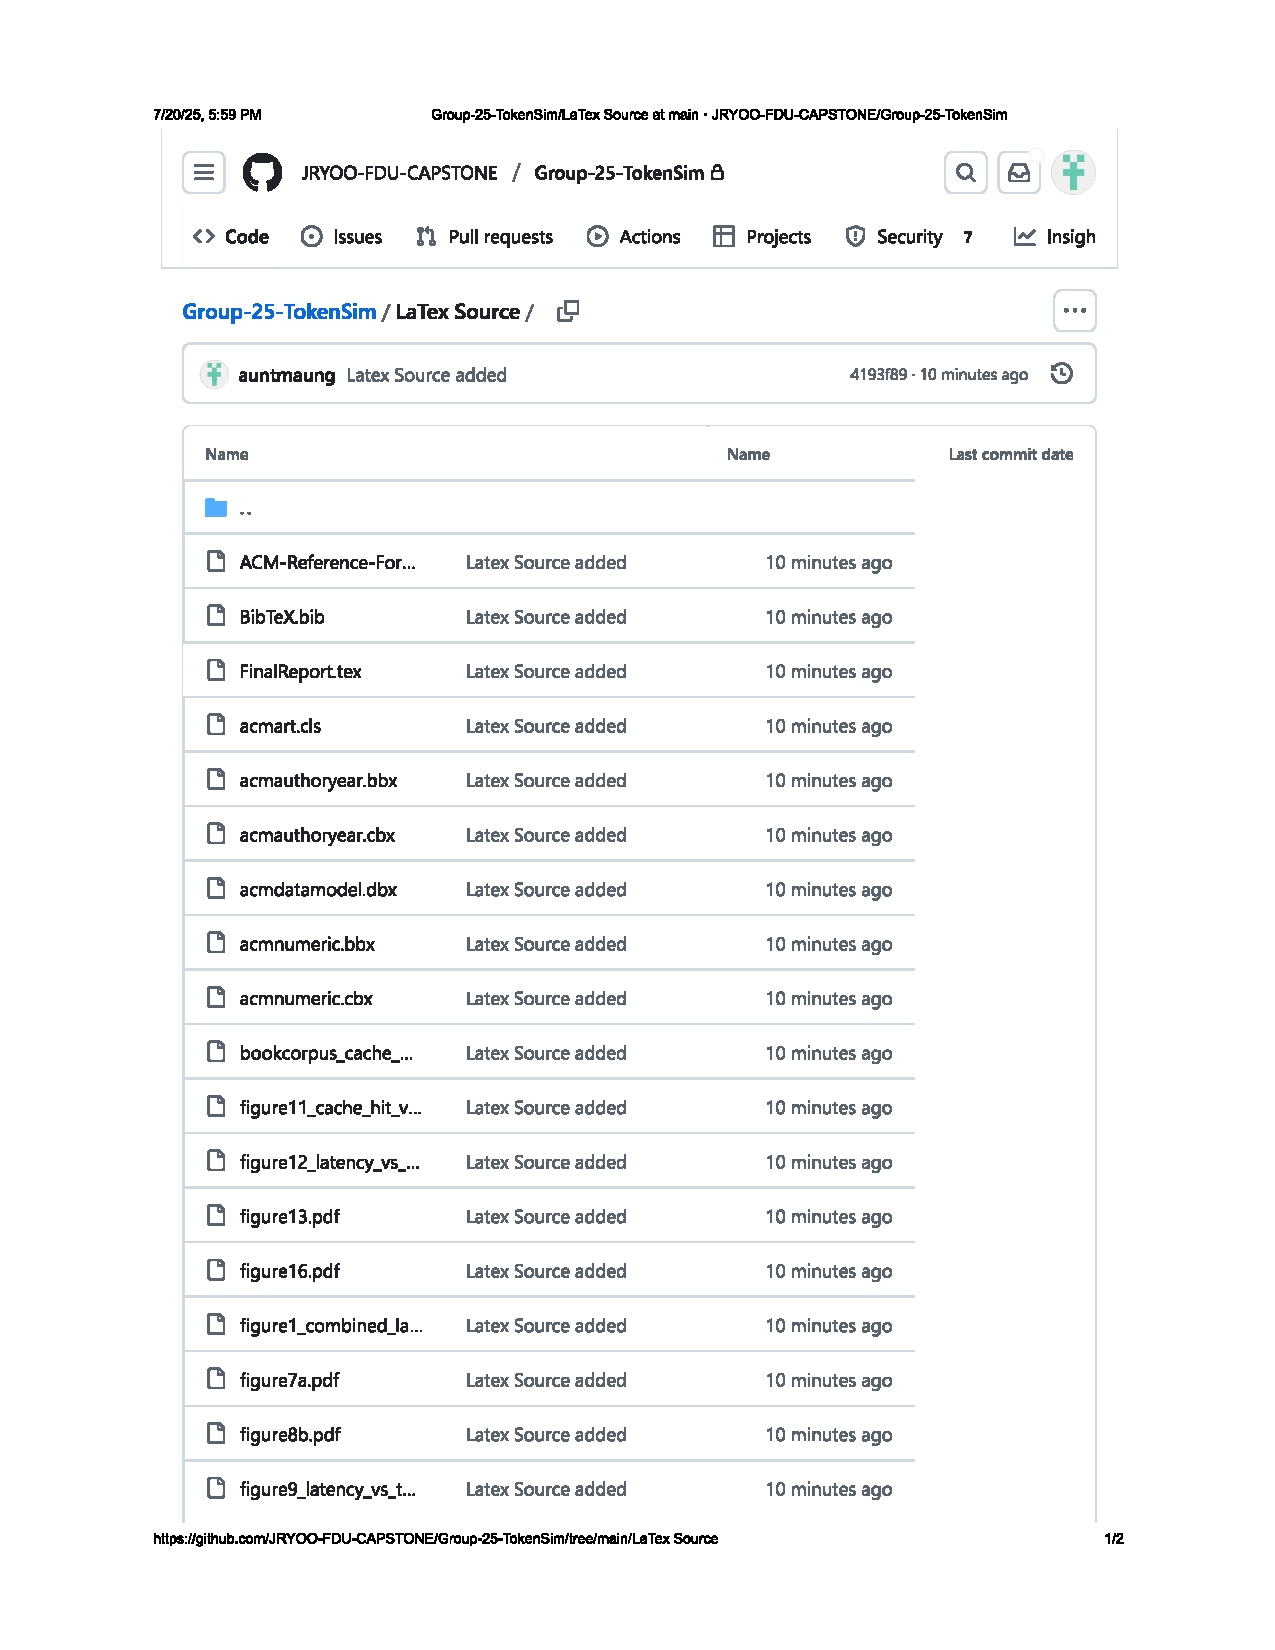
\includegraphics[width=\textwidth]{Latex75.pdf}
    \caption{Screenshot of GitHub repository which shows LaTeX Source Folder}
    \label{LatexGit}
\end{figure*}
 
 

\end{document}
\endinput
%%
%% End of file `sample-sigconf.tex'.
